\documentclass[aps, secnumarabic, balancelastpage, asmath, amssymb, nofootinbib, floatfix,]{revtex4-2}
\usepackage{minted}
\usepackage{graphicx}
\usepackage{float}
\usepackage{caption}
\usepackage{siunitx}
\usepackage[export]{adjustbox}
\usepackage{subcaption}
\usepackage{amsmath}
\usepackage{hyperref}
\usepackage{subcaption}
\usepackage{tikz}
\usepackage{multirow}
% \usepackage[table,xcdraw]{xcolor}
\usepackage{xcolor}
\usepackage{cprotect}
\usepackage{verbatimbox}
\usepackage{listings}
\usepackage{xparse}
\usepackage{listings}
%\usepackage{times}
\NewDocumentCommand{\codeword}{v}{%
\texttt{\textcolor{black}{#1}}%
}

\hypersetup{colorlinks=true, pdfstartview=FitV, linkcolor=blue, citecolor=black, plainpages=false, pdfpagelabels=true, urlcolor=blue}

\newenvironment{code}{\captionsetup{type=listing}}{}
% \SetupFloatingEnvironment{listing}{name=Source Code}

\definecolor{backcolour}{rgb}{0.95,0.95,0.92}
\definecolor{mGreen}{rgb}{0,0.6,0}
\definecolor{mGray}{rgb}{0.5,0.5,0.5}
\definecolor{mPurple}{rgb}{0.58,0,0.82}
\definecolor{backgroundColour}{rgb}{0.95,0.95,0.92}
\definecolor{LightGray}{gray}{0.9}

\setlength{\arrayrulewidth}{0.3mm}
\setlength{\tabcolsep}{5pt}
\renewcommand{\arraystretch}{1.5}
\graphicspath{{./image/}}

\usepackage{setspace}
\usepackage{titletoc}
%\contentsmargin{2.55em}
\dottedcontents{chapter}[1.5em]{}{2.3em}{1pc}
\dottedcontents{section}[1.5em]{}{1.7em}{0.5pc}
\dottedcontents{subsection}[3.9em]{}{2.4em}{0.5pc}
\dottedcontents{subsubsection}[6.6em]{}{2.7em}{0.5pc}
\dottedcontents{paragraph}[9.5em]{}{1.9em}{0.5pc}

\usepackage{etoolbox}
\makeatletter
\pretocmd{\chapter}{addtocontents{toc}{\protect\addvspace{15\p@}}}{}{}
\pretocmd{\section}{\addtocontents{toc}{\protect\addvspace{9\p@}}}{}{}
%\pretocmd{\subsection}{\addtocontents{toc}{\protect\addvspace{15\p@}}}{}{}
\makeatother


\stepcounter{secnumdepth}
\stepcounter{tocdepth}

% Usual (decimal) numbering
\renewcommand{\thesection}{\arabic{section}}
\renewcommand{\thesubsection}{\thesection.\arabic{subsection}}
\renewcommand{\thesubsubsection}{\thesubsection.\arabic{subsubsection}}

% Fix references
\makeatletter
\renewcommand{\p@subsection}{}
\renewcommand{\p@subsubsection}{}
\makeatother

\lstset
{ %Formatting for code in appendix
    basicstyle=\footnotesize,
    numbers=left,
    stepnumber=1,
    showstringspaces=false,
    tabsize=1,
    breaklines=true,
    breakatwhitespace=false,
    %basicstyle=\ttfamily,
    %columns=fullflexible,
    frame=single,
    postbreak=\mbox{\textcolor{red}{$\hookrightarrow$}\space},
    numbersep=5pt,
}

\usepackage{wrapfig}

\begin{document}
%top matter
    \begin{titlepage}
   \begin{center}
       \vspace*{1cm}

	\Huge
       \textbf{CE339 - High Level Digital Design}

       \vspace{0.5cm}
       
       \LARGE
        \textbf{Assignment 2 -- ``Snake'' Video Game}
            
       \vspace{1.5cm}

       \textbf{Akshay Gopinath}\\
       \textbf{Registration Number: 2005614}\\
       \textbf{Word Count: xxxx}\\

       \vfill
        \begin{figure}[h]
        
        
\includegraphics[scale = 0.85]{University}
        
   	\end{figure}
        \vfill
            
       A report presented for the degree of\\
       Electronic Engineering
            
       \vspace{1cm}
     
            
       School of Computer Science and Electronic Engineering\\
       University of Essex\\
       England\\
       \today

   \end{center}
\end{titlepage}

%\thispagestyle{plain}
%\Large
%\textbf{Contributions}

%\clearpage

\thispagestyle{plain}
\begin{center}
    \Large
    \textbf{CE339 - High Level Digital Design}
        
    \vspace{0.4cm}
    \large
    \textbf{Assignment 2 -- ``Snake'' Video Game}
        
    \vspace{0.4cm}
    \textbf{Akshay Gopinath}
       
    %\vspace{0.9cm}
    \section*{Abstract}
    \fontsize{11pt}{12pt}\selectfont
    
\end{center}
\fontsize{11pt}{12pt}\selectfont
{
\setlength{\parindent}{0pt}


}
\clearpage

\tableofcontents

\clearpage

\listoffigures
\clearpage

% \listoftables

\clearpage


\section{\fontsize{11.3pt}{12pt}\selectfont \bf Introduction}
\fontsize{11pt}{12pt}\selectfont
\label{sec:1}

{
\setlength{\parindent}{0pt}

This report documents an experiment to design a ``Snake'' Video Game on hardware using a Hardware Description Language (HDL) called VHDL (Very High Speed Integrated Circuit Hardware Design Language). The target platform is the Digilent Basys3 Board which houses an Artix-7 based FPGA[1]. The VHDL code is synthesised using Xilinx Vivado. The VGA (Video Graphics Array) port on the Basys3 board is used to display the game on a compatible monitor and the player score is shown on the 7-segment display. This report will explain the design in a top-down approach, whilst going into detail on every sub-components. The top level schematic will generate the necessary signals required to correctly display the game and the score, such as the VGA synchronisation signals, RGB (red, green, blue) colour signals and the 7-segment display cathode and anode signals.

\section{\fontsize{11.3pt}{12pt}\selectfont \bf The Design}

\subsection{\fontsize{11.4pt}{12pt}\selectfont \bf High Level Overview \label{sec:2.1}}

\fontsize{11pt}{12pt}\selectfont
\label{sec:2}

\begin{figure}[h]
  \centering
  %\captionsetup{justification=centering}
  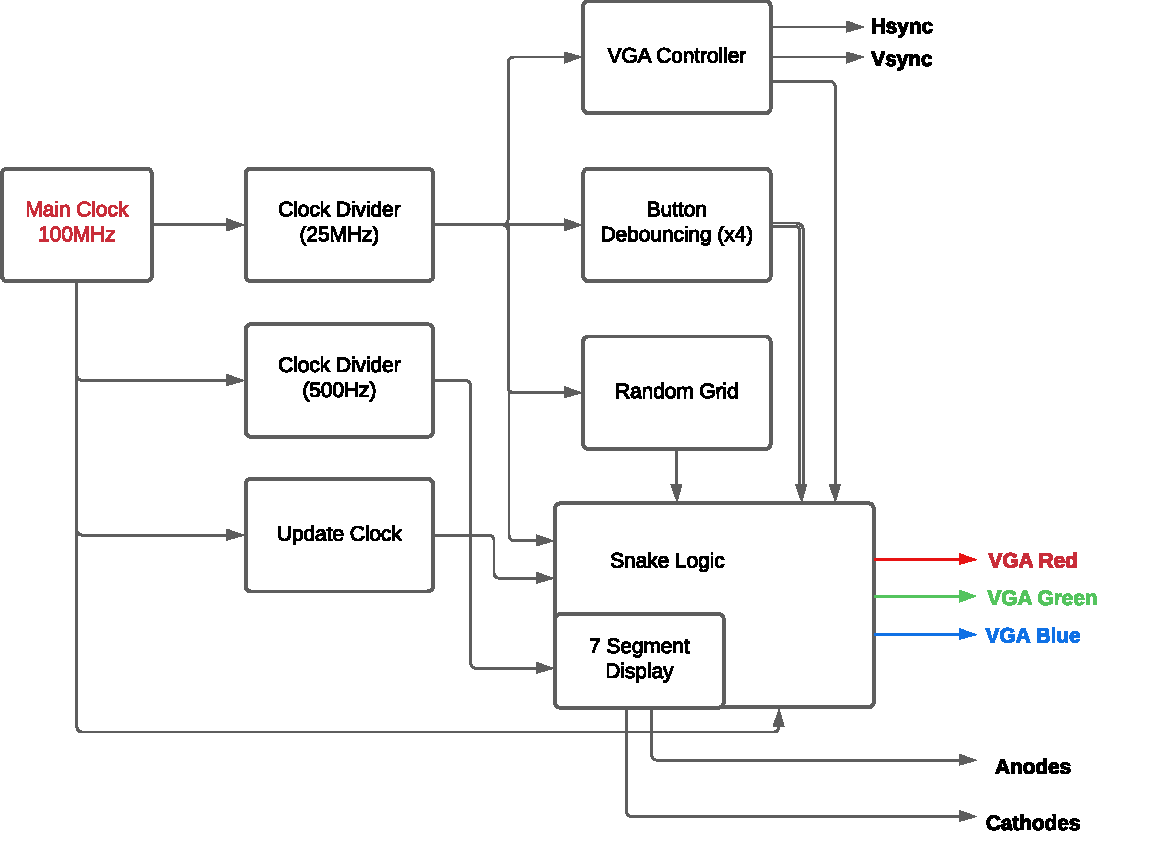
\includegraphics[scale = 0.7]{VGA-Flow - Page 1.pdf}
  \caption{\em High level architecture of the system}
  \label{fig:1}
\end{figure}

Figure \ref{fig:1} above shows the high level block diagram of the system. The main clock is from the Basys3 board which is at 100MHz frequency. The targer resolution is 640x480. The pixel clock is 25MHz, with a refresh rate of 60Hz. In order to generate the required synchronisation signals (by the VGA Controller module) for these specifications, the VGA controller module needs a 25MHz a clock. Hence the 100MHz master clock is given as input to a clock divider to generate this frequency. The 25MHz clock is also used for button debouncing (to keep it in synchronisation with the graphics being rendered to the screen), and also for the Random Grid module. Another clock divider was instantiated to generate a 500Hz clock. The 500Hz clock is used for the time multiplexed 7-segment display driver, which resides inside the Snake Logic module. The update clock is a module used to generate a pulse at a desired frequency (in this case 25Hz), which is high only for one clock cycle of the master clock. The purpose of this module is to set the update frequency of the game logic, hence the output of the update clock is given as input to the Snake Logic module. The Random Grid module is used to generate pseudo random locations for the positions of the food in the game. And the output is given to the Snake Module as input. The VGA Controller module generates the horizontal and vertical synchronisation signals for the VGA Port. It also outputs the current x and y count co-ordinate as well as the blanking signal for the Snake Logic module to keep track of the screen position. The Snake Logic block is the main heart of the system. The Snake Logic module is the heart of the entire system, and contains the game main logic, as well as the rendering signals. This module contains many processes to control game elements such as the snake location direction, snake direction, snake size, game state, game levels etc. The module also contains the 7-segment display driver and BCD (Binary Coded Decimal) counters to display the score whilst playing the game. This module outputs the anode and cathode signals for the 7-segment display as well as the red, green and blue signals for the VGA port. The high level diagram from Figure \ref{fig:1} represents the main top level file shown in \hyperref[code:main]{Source Code 1}.

\vspace{-1.0em}
\subsection{\fontsize{11.4pt}{12pt}\selectfont \bf Detailed Overview \label{sec:2.2}}

\subsubsection{\fontsize{10pt}{12pt}\selectfont \bf snake \label{sec:2.2.1}}

\vspace{-1.5em}
\begin{wrapfigure}[14]{l}{0.6\textwidth}
    \centering
    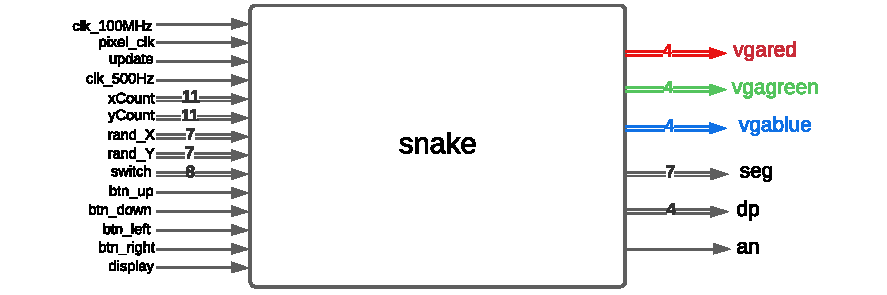
\includegraphics[scale = 0.8]{VGA-Flow - Page 1-1.pdf}
    \caption{\em Inputs/outputs of snake module}
    \label{fig:2}
\end{wrapfigure}

Figure \ref{fig:2} on the left depicts the inputs and outputs of the \verb|snake| module. This module contains the main logic that controls the snake game, as well as the Read Only Memories (ROMs) that store the bitmapped sprites/graphics. The inputs are master 100MHz clock (for synchronisation), pixel clock (25MHz), update clock (25Hz), x and y counters, random food location, and the debounced buttons. It outputs the red, green, blue signals for VGA and the cathode and anode signals for the 7-segment display. 


\begin{figure}[h]
  \centering
  %\captionsetup{justification=centering}
  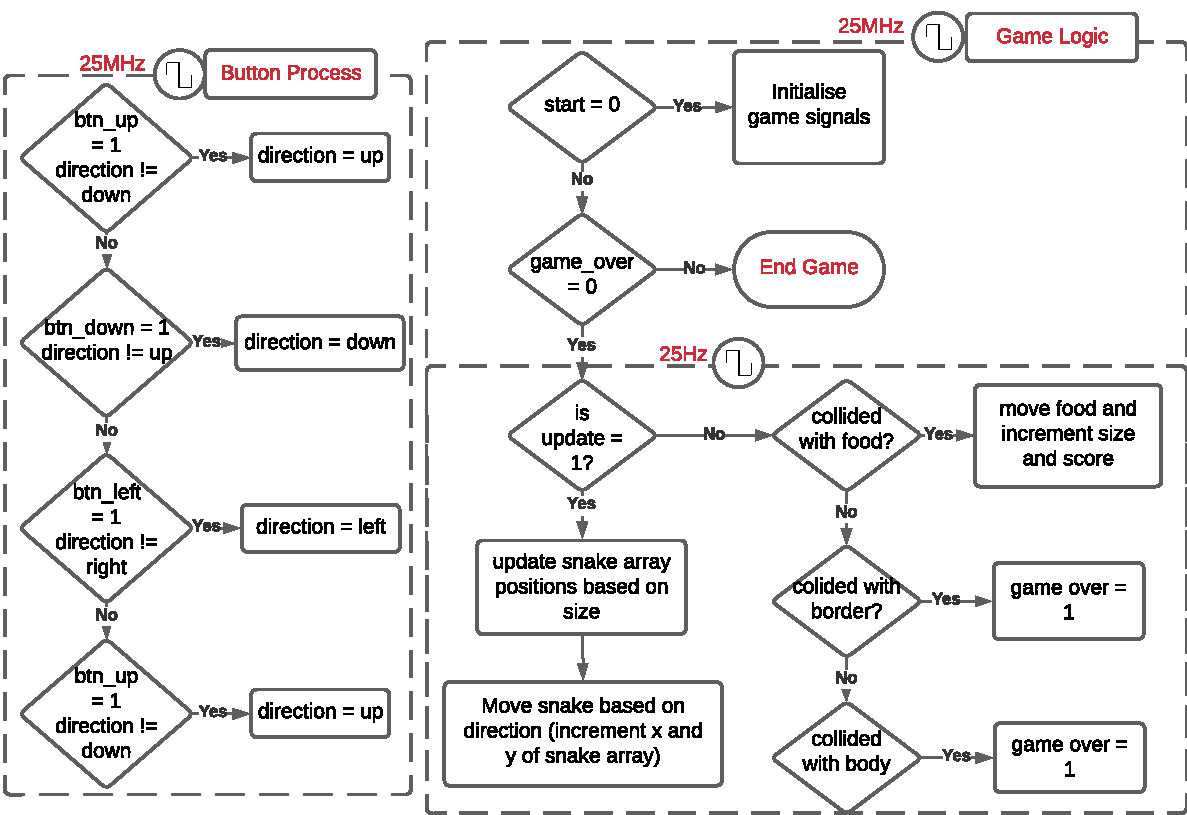
\includegraphics[scale = 0.72]{logic.pdf}
  \caption{\em Button and game logic processes of the snake module}
  \label{fig:3}
\end{figure}

\clearpage

\begin{wrapfigure}[32]{l}{0.5\textwidth}
    \centering
    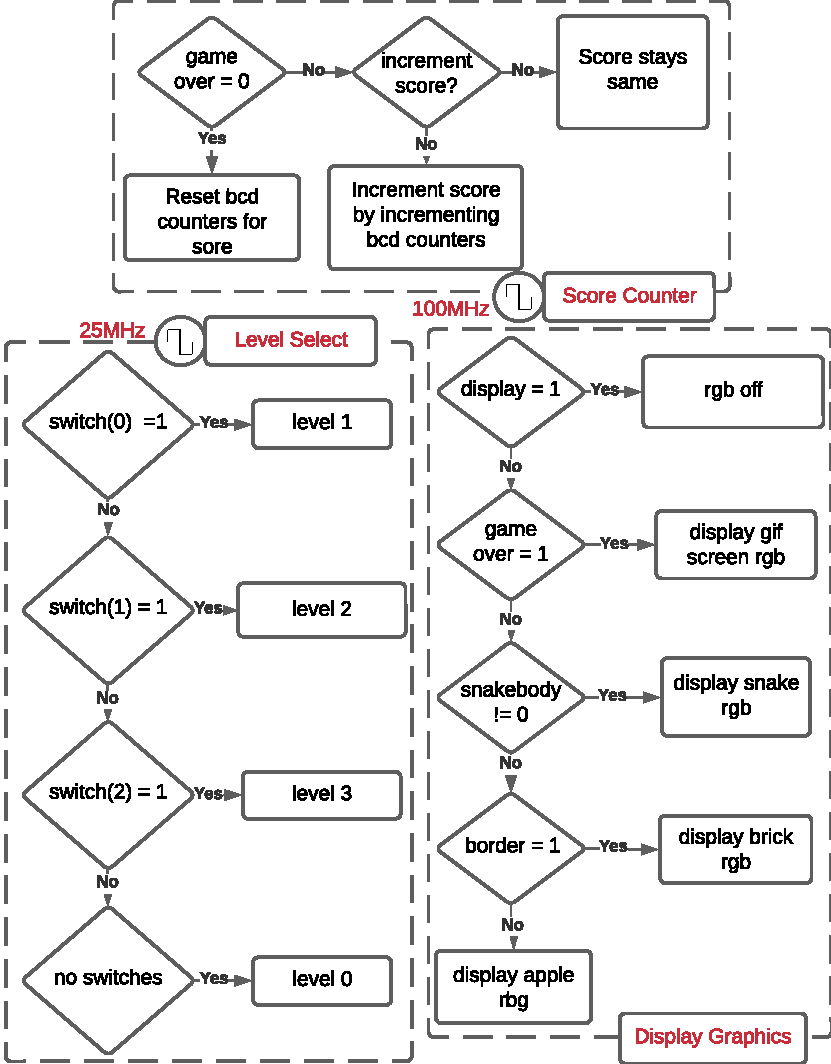
\includegraphics[scale = 0.65]{score.pdf}
    \caption{\em Level select and score count process and colour rendering}
    \label{fig:4}
\end{wrapfigure}

The \verb|snake| module is composed of many processes to construct the game logic and behaviour. Figure \ref{fig:3} and Figure \ref{fig:4} shows flow diagrams to represent this. Figure \ref{fig:3} above shows the button/input and the main game logic process. The button process sets the value of the \verb|direction| register based on the button input. The button input is received from the \verb|Debounce| module (which debounces the button presses for reliability). This process updated with the pixel clock of 25MHz. The game logic process handles updating the snake for the movement as well as checking for collisions. If the start signal is zero, the game is idle and all the starting game conditions are set to defaults (such as initial food location). If the game over signal is high, the game will end until the game is reset, and once reset, the game is reset back to default values. This part of this process is updated at 25MHz. The other parts of the process is updated at 25Hz, which is the games update clock. When the update clock is high, the snake position array (for both x and y locations) are updated in a for loop depending on the current snake size. The snake position at the first index (snake head) is updated depending on the current direction (set by the buttons). When the update clock is low, the collision between the border, food and the snake body is checked. If a collision with the food is detected, the snake size is incremented (unless max snake length is reached). Next if the snake head collides with a border or itself, then the game over signal will be set, thus ending the game, until the game is reset.  Figure \ref{fig:4} shows three other important processes in this module. The score counting process increments the score during the game when food is collected and when the game ends, the game is reset. BCD counters and a 7-segment display driver is used to achieve this. The level select process is very simple, it selects the level based on the switch input. And the levels are border signals that are generated based on certain conditions that decide where the borders are placed on the screen. Lastly, the colour displaying/rendering logic is a combinational process, the other processes we have seen so far are sequential logic. If the display signal is high (same as blanking, which is active low logic), then the RBG colours are turned off. The rgb colours are selected based on which graphics is to be rendered, in this case, the border graphics, the game over GIF and the snake. Graphics in this game are all bitmapped ROMs, this will be explained later in the report. 

\vspace{-1.5em}
\subsubsection{\fontsize{10pt}{12pt}\selectfont \bf updateClk \label{sec:2.2.2}}
\vspace{-1.5em}
% \begin{wrapfigure}[32]{l}{0.5\textwidth}
%     \centering
%     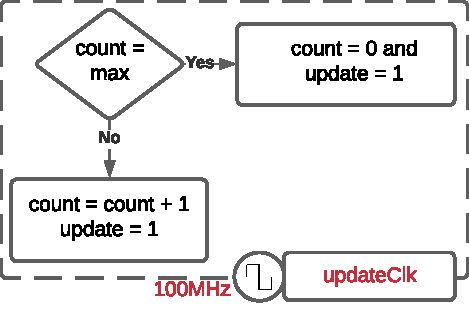
\includegraphics[scale = 0.65]{update.pdf}
%     \caption{\em Level select and score count process and colour rendering}
%     \label{fig:4}
% \end{wrapfigure}

\begin{figure}[h]
\centering
\captionsetup{justification=centering}
\begin{subfigure}{0.5\textwidth}

%   \centering
  %\captionsetup{justification=centering}
  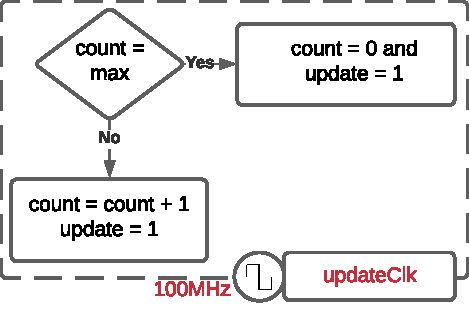
\includegraphics[scale = 0.6]{update.pdf}
  \caption{\em Flow chart for updateClk}

% \caption{\em Diagram of a Differential Drive Mobile Robot}
\label{fig:subim1}
\end{subfigure}
\begin{subfigure}{0.4\textwidth}
%   \centering
  %\captionsetup{justification=centering}
  
\includegraphics[scale = 0.72]{update_block.pdf}
  \caption{\em Entity block of updateClk}
  
% \caption{\em Differential Drive Robot Kinematics}
\label{fig:subim2}
\end{subfigure}
\caption{\em updateClk module diagrams}
\label{fig:5}
\end{figure}

\clearpage

Figure \ref{fig:5} above contains two sub figures, Figure \ref{fig:subim1} and Figure \ref{fig:subim2} which are the architecture and block diagram of this entity respectively. This module has one input, the master clock and one output, the update clock. This is a generic value where the max count can be configured for a different update clock. The update clock used in this game is set to 25Hz. The architecture counts till the set max value and sets the output high for one clock cycle of the master clock, and then becomes low after.

\vspace{-1em}
\subsubsection{\fontsize{10pt}{12pt}\selectfont \bf randomGrid \label{sec:2.2.3}}


\vspace{-1.5em}
\begin{wrapfigure}[7]{l}{0.4\textwidth}
    \centering
    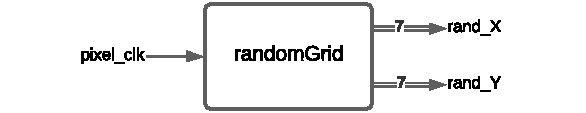
\includegraphics[scale = 0.85]{random.pdf}
    \caption{\em randomGrid entity diagram}
    \label{fig:6}
\end{wrapfigure}
~\\
Figure \ref{fig:6} on the left shows the inputs and outputs of the randomGrid module. This module is used to generate the pseudo random x and y locations for the food. The pseudo random generation implementation in this project is very simple, as a simple mathematical operation is done on the current random location to move the food `unprediectably'.

\begin{code}
  \label{code:1}
  \captionof*{listing}{Code Snippet 1: {randomGrid architecture implementation}}
  \vspace{-0.5em}
  \begin{minted}
  [
  frame=single,
  framesep=10pt,
  baselinestretch=1.2,
  bgcolor=backgroundColour,
  fontsize={\fontsize{9.5}{6.5}\selectfont},
  % linenos,
  tabsize=2,
  breaklines
  ]
  {vhdl}
if rising_edge(pixel_clk) then
    rand_X <= ((rand_X + 3) mod 37) + 1; -- set random x and y position
    rand_Y <= ((rand_Y + 3) mod 27) + 1;
end if;
  \end{minted}
  \end{code}
  
Since the implementation is simple, it is shown in \hyperref[code:1]{Code Snippet 1}. A simple arithmetic oprtation is computed on the value read back from the current random x and y value, at the rising egde of the pixel clock. The output of this module is given as input to the \verb|snake| module.

\vspace{-1.5em}
\subsubsection{\fontsize{10pt}{12pt}\selectfont \bf 7-Segment Display \label{sec:2.2.4}}

\begin{figure}[h]
  \centering
  %\captionsetup{justification=centering}
  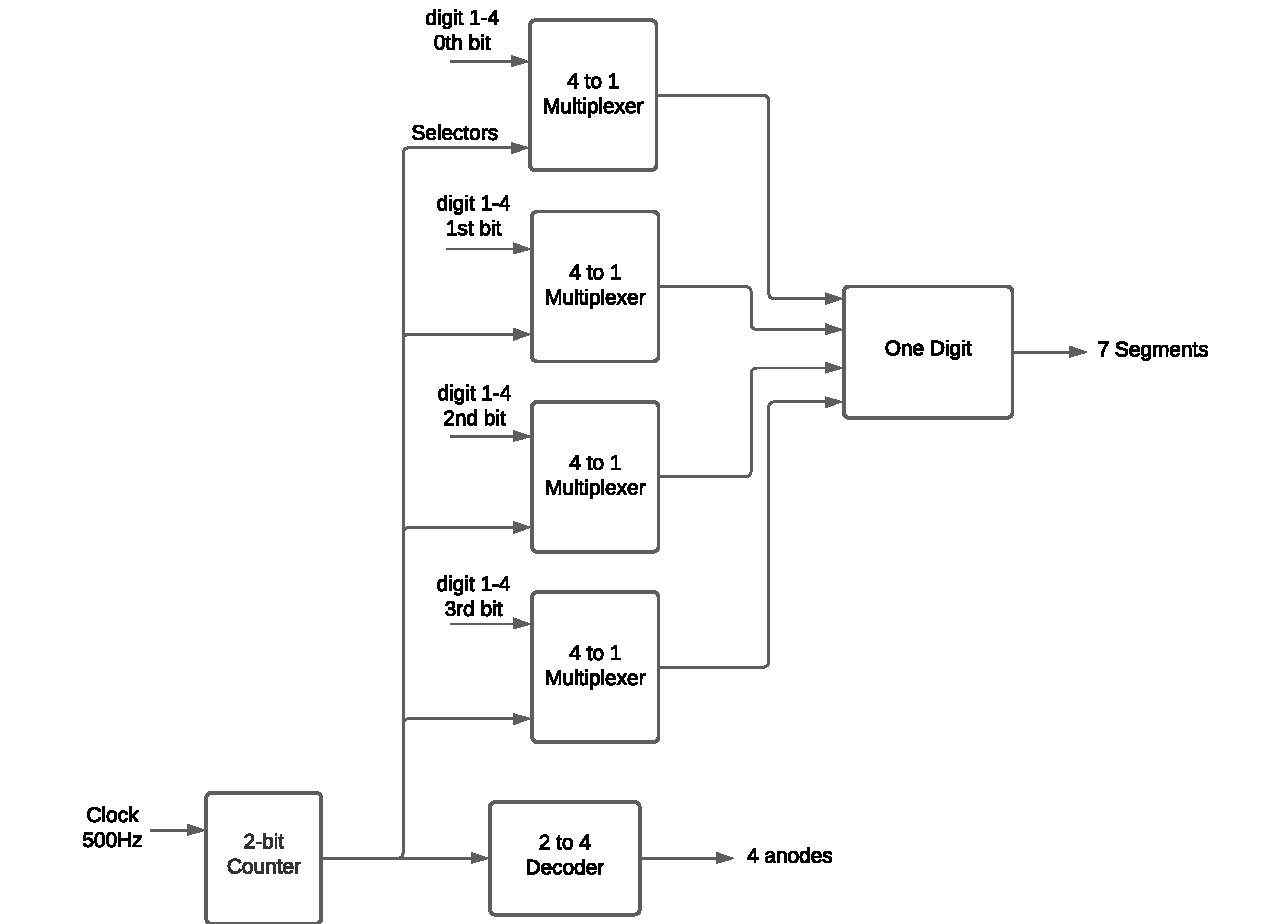
\includegraphics[scale = 0.69]{four_digits.pdf}
  \caption{\em Architectural block diagram of the four\_digits module}
  \label{fig:7}
\end{figure}

\clearpage

\begin{wrapfigure}[9]{l}{0.42\textwidth}
  \centering
  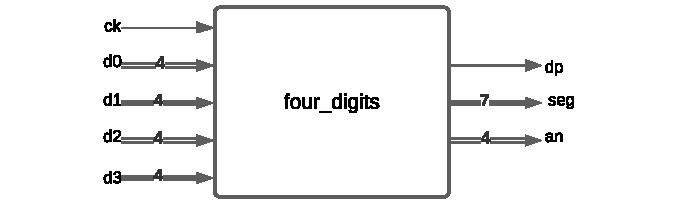
\includegraphics[scale = 0.8]{four_digit_block.pdf}
  \caption{\em four\_digits entity diagram}
  \label{fig:8}
\end{wrapfigure}

This section explains the 7-segment display driver (and it's subcomponents) circuit used to display the score. Figure \ref{fig:8} on the left shows the entity inputs and outputs and Figure \ref{fig:7} above shows the high level connection diagram. This module takes in a 500Hz clock, and four inputs which are four bits wide, and generates the required anode and cathode displays. Time division multiplexing is used to display the four digits on the four seven segment displays available on the Basys3 board. The 500Hz clock given to a two bit counter which counts from 0$\rightarrow$3, and it's output is fed into a 4-t0-1 multiplexer to select the corresponding bit for that digit. The four multiplexer output is given to a module called \verb|one_digit| which is a 7-segment decoder. The 2-bit counter output is also used by a 2-to-4 decoder to select the correct anode which is currently being displayed. The anodes are swapped at a rate of 500Hz, a refresh rate human eyes cannot visibly see. The 2-bit counter being very simple is implemented using behavioural modelling. Figure \ref{fig:9}, \ref{fig:10} and \ref{fig:11} below shows the entity block diagrams of \verb|mux4_1|, \verb|decoder2_4| and \verb|one_digit| respectively, which is used in the circuit from Figure \ref{fig:7}.

\begin{figure}[!htb]
  \minipage{0.32\textwidth}
    
\includegraphics[width=\linewidth]{mux4.pdf}
    \caption{\em mux4\_1 entity}\label{fig:9}
  \endminipage\hfill
  \minipage{0.32\textwidth}
    
\includegraphics[width=\linewidth]{dec.pdf}
    \caption{\em decoder\_2\_4 entity}\label{fig:10}
  \endminipage\hfill
  \minipage{0.32\textwidth}%
    
\includegraphics[width=\linewidth]{one_digit.pdf}
    \caption{one\_digit entity}\label{fig:11}
  \endminipage
  \end{figure}
  
All the three modules are very simple. \verb|one_digit| takes in a 4 bit number as input and outputs the corresponding 7 bit output for the 7 segments on the 7-segment display. The \verb|decoder| entity is a simple two-to-four decoder, a certain bit of the 4 bit output is low depending on the input. For example, if the input is $01_2$, the output is $1101_2$, the $2^{\text{nd}}$ bit is low. And lastly, the 4-to-1 mux routes the corresponding bit of the input \verb|a| depending on the select input \verb|s|, to the output. The \verb|four_digit| module is instantiated inside the \verb|snake| module from Figure \ref{fig:2} and its outputs are propagated outside the \verb|snake| module.

\vspace{-1em}
\subsubsection{\fontsize{10pt}{12pt}\selectfont \bf Debounce \label{sec:2.2.5}}

\begin{figure}[h]
\centering
\captionsetup{justification=centering}
\begin{subfigure}{0.5\textwidth}

%   \centering
  %\captionsetup{justification=centering}
  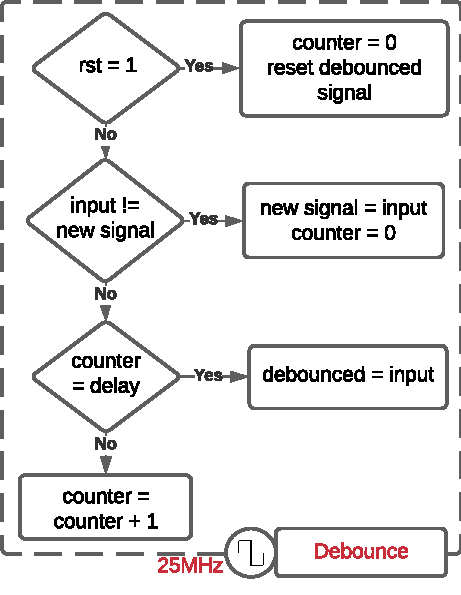
\includegraphics[scale = 0.6]{debounce_flow.pdf}
  \caption{\em Flow chart for Debounce}

% \caption{\em Diagram of a Differential Drive Mobile Robot}
\label{fig:subim3}
\end{subfigure}
\begin{subfigure}{0.4\textwidth}
%   \centering
  %\captionsetup{justification=centering}
  
\includegraphics[scale = 0.72]{debounce.pdf}
  \caption{\em Entity block of Debounce}
  
% \caption{\em Differential Drive Robot Kinematics}
\label{fig:subim4}
\end{subfigure}
\caption{\em Debounce module diagrams}
\label{fig:12}
\end{figure}

Figure \ref{fig:subim3} and \ref{fig:subim4} shows the flow chart and entity diagram for the Debounce module respectively. There are three inputs, clk, rst and noisy (the button input) and one output which is thd debounced press. This module has a configurable generic parameter, \verb|DELAY|. This module is clocked at the pixel clock, 25MHz. The module has a counter that counts till a delay value is reached, and once the count is same as the delay, the button press is debounced, and the counter is reset. The debounced output is input to the \verb|snake| module.

\clearpage

\subsubsection{\fontsize{10pt}{12pt}\selectfont \bf vga\_controller\_640\_60 \label{sec:2.2.6}}


\vspace{-1.5em}
\begin{wrapfigure}[10]{l}{0.45\textwidth}
    \centering
    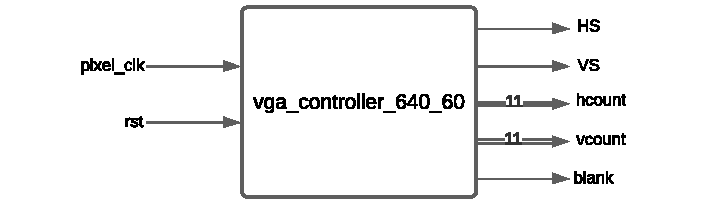
\includegraphics[scale = 0.8]{vga_controller.pdf}
    \caption{\em VGA Controller module}
    \label{fig:13}
\end{wrapfigure}
~\\
Figure \ref{fig:13} on the left shows the entity diagram of the \verb|vga_controller_60_40| module. This module wasn't written by the author and was given by the supervisor. This module has 2 inputs, the 25MHz pixel clock (\verb|pixel_clock|) and reset (\verb|rst|). And outputs the horizontal sync (\verb|HS|), vertical sync \verb|VS|, current horizontal counter value (\verb|hcount|), current vertical counter value (\verb|vcount|) and the blanking signal (\verb|blank|). The horizontal and vertical synchronisation signals are outputted to the VGA port in the top level hierarchy. The vertical counter, horizontal counter and the blanking signals are all given as inputs to the \verb|snake| module from \ref{fig:2} to control the game logic.

\vspace{-1em}
\subsubsection{\fontsize{10pt}{12pt}\selectfont \bf nbit\_clk\_div \label{sec:2.2.7}}
\vspace{-0.5em}
\begin{figure}[h]
\centering
\captionsetup{justification=centering}
\begin{subfigure}{0.5\textwidth}

%   \centering
  %\captionsetup{justification=centering}
  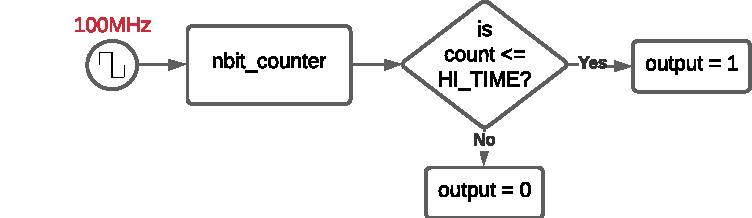
\includegraphics[scale = 0.6]{clk-block.pdf}
  \caption{\em Flow chart for nbit\_clk\_div}

% \caption{\em Diagram of a Differential Drive Mobile Robot}
\label{fig:subim5}
\end{subfigure}
\begin{subfigure}{0.4\textwidth}
%   \centering
  %\captionsetup{justification=centering}
  
\includegraphics[scale = 0.72]{clk_div.pdf}
  \caption{\em Entity block of nbit\_clk\_div}
  
% \caption{\em Differential Drive Robot Kinematics}
\label{fig:subim6}
\end{subfigure}
\caption{\em nbit\_clk\_div module diagrams}
\label{fig:14}
\end{figure}

Figure \ref{fig:14} above shows the flow diagram and entity diagram of the \verb|nbit_clk_div| module (Figure \ref{fig:subim5} and \ref{fig:subim6} respectively). There is one input, the clock and one output, the divided clock. This module is a configurable and generic which is configurable, such as the division factor and the duty cycle. This is possible because the module instantiates another module called \verb|nbit_counter| inside it, which also a generic component. The counter is clocked at 100Mhz (the master clock) and the output is compared with the configured highest count. If the counter reaches a value within a certain threshold, it makes the output high, else makes it low. And the constant \verb|HI_TIME| is calculated from a generic value \verb|high_count|, to control the duty cycle as per the user's usage.

\begin{wrapfigure}[7]{l}{0.35\textwidth}
    \centering
    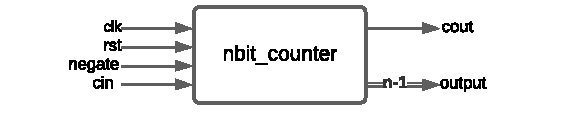
\includegraphics[scale = 0.8]{counter.pdf}
    \caption{\em nbit\_counter module}
    \label{fig:15}
\end{wrapfigure}
~\\
Figure \ref{fig:15} on the left-hand side shows the generic counter used inside the clock divider. It has a configurable maximum count value. It is a very general purpose module as it has a \verb|negate| input, and the \verb|cin| input and \verb|cout| output can be used to easily chain multiple counters. The output of this module is used in the clock divider module in order to generate the divided clock signal. 

\vspace{-1em}
\subsubsection{\fontsize{10pt}{12pt}\selectfont \bf nbit\_bcd\_counter \label{sec:2.2.8}}

\vspace{-1em}
\begin{wrapfigure}[7]{l}{0.37\textwidth}
  \centering
  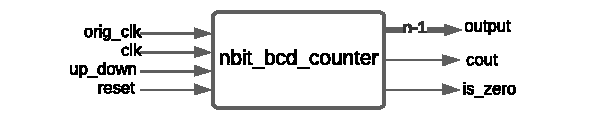
\includegraphics[scale = 0.8]{bcd.pdf}
  \caption{\em nbit\_bcd\_counter module}
  \label{fig:16}
\end{wrapfigure}
~\\
Figure \ref{fig:16} on the left shows the entity block diagram of the \verb|nbit_bcd_counter| module, which is a generic BCD counter which is configurable from a maximum count between 0$\rightarrow$99. This module is used to keep track of the score as the snake eats the food objects. The implementation of this module is very simple, inside it are two modulo-10 counters that are cascaded. When one modulo-10 counter reaches it's $1001_2$ (in up count) or $0000_2$ (in down count), the second counter is incremented or decremented respectively. There are 3 inputs, the original master clock (\verb|orig_clk|, to help with synchronisation), the clock (\verb|clk|) at which the counter is incremented, \verb|up_down| to swap between up and down count mode, and \verb|reset|. The \verb|is_zero| output is not used. This module is instantiated inside the \verb|snake| module, and two are instantiated (as there are 4 7-segment displays) and are cascaded using the \verb|cout| output. The output of the 2 BCD counters are inputs to the \verb|four_digits| module.

\clearpage

\subsubsection{\fontsize{10pt}{12pt}\selectfont \bf Bitmapped Sprites and GIFs \label{sec:2.2.9}}

As mentioned in section \ref{sec:2.2.1} of this report, graphics used in this game are stored as bitmap ROMs. This section details how sprites as well as GIFs were rendered on the VGA monitor. Bitmaps were used to render sprites and GIFs on the screen. A bitmap is essentially an array that holds information for each pixel in the image. In the case of this design, each element in the array holds RGB colour value for each pixel. 

\begin{code}
  \label{code:2}
  \captionof*{listing}{Code Snippet 2: {\em ROM used for the snake sprite}}
  \vspace{-0.5em}
  \begin{minted}
  [
  frame=single,
  framesep=10pt,
  baselinestretch=1.2,
  bgcolor=backgroundColour,
  fontsize={\fontsize{7.5}{6.5}\selectfont},
  % linenos,
  tabsize=2,
  breaklines
  ]
  {vhdl}
type color_sprite_8 is array (0 to 7, 0 to 7) of std_logic_vector(0 to 11);
constant SNAKE_ROM : color_sprite_8 := (
	("010101100010","011010000010","011010000010","011010000010","011010000010","011010000010","011010000010","001001010001"),
	("011010000010","010011000001","001110110001","001110110001","001110110001","001110110001","001110110001","001001100001"),
	("011010000010","001110110001","000110100001","000110100000","000110100000","000110100001","000110100000","001001100001"),
	("011010000010","001110110001","000101110001","001010100001","001010100001","001001110001","001010100001","001001100001"),
	("011010000010","001110110001","000110100001","001010010001","001010010001","001010100001","001010110000","001001100001"),
	("011010000010","001110110001","000110100001","001010100001","001010100001","001010100001","001010110000","001001100001"),
	("011010000010","001110110001","000110110000","001010110000","001010110000","001010110000","001010110000","001001100001"),
	("001001010001","001001100001","001001100001","001001100001","001001100001","001001100001","001001100001","000101010001")
);
  \end{minted}
  \end{code}

\hyperref[code:2]{Code Snippet 2} above shows the ROM implemented to display the snake sprite. A sprite ROM is essentially a two dimensional array where the width and height represents the size of the sprite. In this case it is eight by eight. And each element is an RGB colour value. The ROM is indexed using the x and y counter values, and then is rendered at the desired location. Rendering static sprites is very simple, but it gets slightly tricky when trying to render animated sprites. An animated sprite contains multiple images, hence the bitmap array is an array of two-dimensional arrays.

\begin{code}
  \label{code:3}
  \captionof*{listing}{Code Snippet 3: {\em Type definition for a GIF with 2 frames}}
  \vspace{-0.5em}
  \begin{minted}
  [
  frame=single,
  framesep=10pt,
  baselinestretch=1.2,
  bgcolor=backgroundColour,
  fontsize={\fontsize{8.5}{6.5}\selectfont},
  % linenos,
  tabsize=2,
  breaklines
  ]
  {vhdl}
type apple_gif_sprite is array (0 to 1, 0 to 15, 0 to 15) of std_logic_vector(0 to 11);
  \end{minted}
  \end{code}

Due to page space constraints, only the type definition is shown in \hyperref[code:3]{Code Snippet 3} above. The above syntax defines a 16 by 16 sprite with 2 frames. And in this case, both the frame and the individual pixel colour in the bitmap needs to be indexed. A simple counter signal is used to index the current frame of the animated sprite. Within the current frame, the x and y counter values are used to get the RGB colour value.\\
These bit maps are generated by a Python script which takes in a GIF or PNG and generates VHDL ROM syntax. Which is then included in the code. All the ROMS are stored in the file \verb|snake.vhd| which is shown in \hyperref[code:snake]{Source Code 2} in the \hyperref[sec:app]{Appendix}.. And the python script is in \hyperref[code:py]{Source Code 13} in the \hyperref[sec:app]{Appendix} as well.

\vspace{-0.7em}
\subsection{\fontsize{11.4pt}{12pt}\selectfont \bf Development Process \label{sec:2.3}}

This section describes the steps taken to develop the hardware design as well as what issues were faced and how they were rectified. First, the given VGA driver source code and simple colour rendering was tested, by attempting to display a solid red colour. This can be seen in the GitLab commit linked \href{https://cseegit.essex.ac.uk/23-24-ce339/23-24_CE339_gopinath_akshay/-/commit/41b12159ecd4fd75b2ae10749d8d0f7c15da76b0}{here}. \\
\\
After this, the main snake game logic was developed. As seen from this \href{https://cseegit.essex.ac.uk/23-24-ce339/23-24_CE339_gopinath_akshay/-/commit/911c4fae4d40bebe5094a92a998859baa51b185a}{GitLab commit} link, the colour rendering was not working initially, and some attempts were made to try and rectify this problem. The first attempt was to try making the sequential logic more reliable by following the discussion shown in reference [7]. Apparently in VHDL, it is better to synchronise most logic to the master clock of the board (thus rising edge of the 100MHz clock), and use the output of the clock divider as an enabler signal. This is because the synthesiser interprets the output of a clock divider as a normal `wire' and not as a `clock'. Although this didn't fix the issue after \href{https://cseegit.essex.ac.uk/23-24-ce339/23-24_CE339_gopinath_akshay/-/commit/18064c441e06b2e87fbe97886cf5f8ecc04e3233}{this commit}, this is a good VHDL coding practice regardless. This issue was later rectified in \href{https://cseegit.essex.ac.uk/23-24-ce339/23-24_CE339_gopinath_akshay/-/commit/08e170dc860f38bff83c3967aa89f9bca4223632}{this commit}. Where in the render logic for the border, an \verb|or| logic was used instead of \verb|and| logic. Which was a silly mistake. Another fix was made in the same commit, where the movement logic was fixed because the x and y movement of the snake was inverted. \\
~\\
The next  bug discovered was that the game would randomly end (game over) whilst the snake was in motion. This was initally beleived to be a synchronisation problem, but the input process was already clocked to the master clock (with the pixel clock as an enabler). To fix this issue, a button debouncing module was created in \href{https://cseegit.essex.ac.uk/23-24-ce339/23-24_CE339_gopinath_akshay/-/commit/2c20b371731b9e364c1e1e8525bab0f203cde461}{this commit}. But not all the buttons were connected to this module. This bug was fixed in \href{https://cseegit.essex.ac.uk/23-24-ce339/23-24_CE339_gopinath_akshay/-/commit/9eff36c14714be44cf6d5e24563ecbe0abaf9896}{this commit} when all four movement buttons were debounced using the module. This highlights the importance of debouncing button presses. \\

Next, rendering sprites and more complex graphics was attempted. First monochrome sprite rendering was attempted, and as seen from \href{https://cseegit.essex.ac.uk/23-24-ce339/23-24_CE339_gopinath_akshay/-/commit/a958a1af9c4bc434596a061d44baa802a9002064}{this commit}, it wasn't working properly on the first try. The sprite appeared to be enlarged and had to be resized. This was later rectified in a \href{https://cseegit.essex.ac.uk/23-24-ce339/23-24_CE339_gopinath_akshay/-/commit/f787fa3ce0e1d44e9f0805a759b5dafe5140fda9}{later commit}, when the rendering logic was given a context of the size of the image rather than using bit splicing. After this was fixed, coloured sprite rendering was added, as seen from \href{https://cseegit.essex.ac.uk/23-24-ce339/23-24_CE339_gopinath_akshay/-/commit/4a8f2602f10cfca06351e9e81d6a3dccfbe525a5}{this commit}. The RGB rendering logic had to be modified, so that there is one signal for colour that can be spliced to separate signals. After a sprite was added for the borders, one more fixed had to be added for the first level of the game, as shown in \href{https://cseegit.essex.ac.uk/23-24-ce339/23-24_CE339_gopinath_akshay/-/commit/72ade113022557aec48fa33dec5331c03ee3bdc1}{this commit}. Where the first level border generation border signal had to have a context of the sprite size. Lastly, the apple and game over screen GIFs were added. Since the logic for this was exactly the same, this worked as expected on the first attempt. ~\\

To understand how to render complex on an FPGA, the website from reference [6] was used. This website teaches the design approach in SystemVerilog rather than VHDL, but all the concepts depicted in the website carried over nicely, and the logic and theory was easily translatable to VHDL. ~\\

The sprite texture used for the food is shown in reference [2], for the brick/border in reference [3] and for the snake body in reference [4].

\vspace{-0.5em}
\subsection{\fontsize{11.4pt}{12pt}\selectfont \bf Possible Design Improvements \label{sec:2.4}}

There are many places where the current hardware design can be improved. For example the current pseudo random location generation uses a very simple arithmetic operation to `randomise' the location of the food. A smarter approach would have been to use a Linear Feedback Shift Register design as shown in reference [7], which is a very popular approach in both hardware and software to generate random numbers. The current apprach was chosen due to simplicity, and works well. And also due to time contraints for the project. ~\\
~\\
The next improvement that could be made with more time is the visuals of the game. The snake sprite could have been animated and also add a textured background to the game, rather than a solid black background. This was not done again due to time constraints but this shouldn't be hard to adapt into the current code base, as rendering sprites and even animated GIFs has been achieved in this project. ~\\
~\\
The snake source code shown in \hyperref[code:snake]{Source Code 2} could also be improved. As all the ROMs are stored in this one file, it makes the file rather large in terms of lines of code. The ROMs could have possibly been stored elsewhere, maybe a separate entity. This would improve code reliability.



\clearpage


\section{\fontsize{11.3pt}{12pt}\selectfont \bf Testing and Final Results}
\fontsize{11pt}{12pt}\selectfont \label{sec:3}








% \section{\fontsize{11.3pt}{12pt}\selectfont \bf Conclusion}
% \fontsize{11pt}{12pt}\selectfont \label{sec:4}




% \section{\fontsize{11.3pt}{12pt}\selectfont \bf References}
% \fontsize{11pt}{12pt}\selectfont \label{sec:5}



% \section{\fontsize{11.3pt}{12pt}\selectfont \bf Appendix}
% \fontsize{11pt}{12pt}\selectfont \label{sec:app}


}

\end{document}

%% [1] https://digilent.com/reference/programmable-logic/basys-3/start
% [2] apple sprite
% [3] brick sprite
% [4] snake sprite
% [5] LSFR https://en.wikipedia.org/wiki/Linear-feedback_shift_register
% [6] fpga project website
% [7] https://stackoverflow.com/questions/19708301/making-a-clock-divider